%LaTeX template : http://systbio.org/files/SB_LaTeX_Template_txt_extension.txt
%Author instructions: http://www.oxfordjournals.org/our_journals/sysbio/for_authors/ms_preparation.html

\documentclass[12pt,letterpaper]{article}
\usepackage{natbib}

%Packages
\usepackage{pdflscape}
\usepackage{fixltx2e}
\usepackage{textcomp}
\usepackage{fullpage}
\usepackage{float}
\usepackage{latexsym}
\usepackage{url}
\usepackage{epsfig}
\usepackage{graphicx}
\usepackage{amssymb}
\usepackage{amsmath}
\usepackage{bm}
\usepackage{array}
\usepackage[version=3]{mhchem}
\usepackage{ifthen}
\usepackage{caption}
\usepackage{hyperref}
\usepackage{amsthm}
\usepackage{amstext}
\usepackage{enumerate}
\usepackage[osf]{mathpazo}
\usepackage{dcolumn}
\usepackage{lineno}
\usepackage{dcolumn}
\newcolumntype{d}[1]{D{.}{.}{#1}}

\pagenumbering{arabic}


%Pagination style and stuff
\linespread{2}
\raggedright
\setlength{\parindent}{0.5in}
\setcounter{secnumdepth}{0} 
\renewcommand{\section}[1]{%
\bigskip
\begin{center}
\begin{Large}
\normalfont\scshape #1
\medskip
\end{Large}
\end{center}}
\renewcommand{\subsection}[1]{%
\bigskip
\begin{center}
\begin{large}
\normalfont\itshape #1
\end{large}
\end{center}}
\renewcommand{\subsubsection}[1]{%
\vspace{2ex}
\noindent
\textit{#1.}---}
\renewcommand{\tableofcontents}{}
%\bibpunct{(}{)}{;}{a}{}{,}

%---------------------------------------------
%
%       START
%
%---------------------------------------------

%Submitting to: Evolution (thorough method + applied data)
%               Proc B (nice story + thorough method in the supplementaries?)
%               MEE (new method (time slicing) + increment on former methods (disparity)) 

% NC: Make sure to format for whichever journal we choose...

\begin{document}

%Running head
\begin{flushright}
Version dated: \today
\end{flushright}
\bigskip
\noindent RH: Tempo and mode in mammalian evolution

\bigskip
\medskip
\begin{center}

\noindent{\Large \bf Cretaceous-Palaeogene extinction does not affect mammalian disparity.} 
% NC: still think this might need some work

\bigskip

\noindent {\normalsize \sc Thomas Guillerme$^1$$^,$$^2$$^*$, and Natalie Cooper$^1$$^,$$^2$$^,$$^3$}\\
\noindent {\small \it 
$^1$School of Natural Sciences, Trinity College Dublin, Dublin 2, Ireland.\\
$^2$Trinity Centre for Biodiversity Research, Trinity College Dublin, Dublin 2, Ireland.\\
$^3$Department of Life Sciences, Natural History Museum, Cromwell Road, London, SW7 5BD, UK.}\\
\end{center}
\medskip
\noindent{*\bf Corresponding author.} \textit{Zoology Building, Trinity College Dublin, Dublin 2, Ireland; E-mail: guillert@tcd.ie; Fax: +353 1 6778094; Tel: +353 1 896 2571.}\\
\vspace{1in}

%Line numbering
\modulolinenumbers[1]
\linenumbers

%---------------------------------------------
%
%       ABSTRACT
%
%---------------------------------------------

\newpage
\begin{abstract}
% NC: As ever I'm ignoring this until we are finished with the rest!
%Massive global extinctions have a turn-over effect on biodiversity. When some large group of taxa suffers from a high rate of extinction, it is expected that niches becomes available for potentially unrelated clades that can undergo an adaptive radiation to fill these vacant niches.
%Therefore, in a context of current global biotic and abiotic changes, resolving this question is crucial to understand the effect of mass extinction events on biodiversity.
%The causes and effects of such events are well understood for marine organisms with a good fossil record (e.g. Ammonoidea and Foraminifera) but the effects remains unclear on some iconic vertebrate groups.

%Typically, placental mammals (eutherians) are shown by some studies to be undergoing an adaptive radiation after the Cretaceous-Palaeogene mass extinction event (K-Pg) by originating shortly before the K-Pg event and displaying high morphological evolutionary rates leading to high diversification during the Palaeogene. However, some other studies have demonstrated that eutherians originates during the Cretaceous and don't display significantly high diversification after the K-Pg event.

%Here we propose a new approach to test if eutherians undergo an adaptive radiation after the K-Pg event. We use trees containing both living and fossil taxa based on all the available data (Total Evidence) and the state-of-the-art method in dating (tip dating) along side with a better proxy for niche occupancy (morphological diversity as opposed to taxonomic diversity) and finer grain analysis through time (introducing a time slicing method).

%Our results shows that eutherians don't display significantly higher changes in morphological disparity that expected under a Brownian motion after the K-Pg boundary. We therefore propose that eutherian mammals don't undergo an adaptive radiation during the Palaeogene.

%Why is our stuff better?
%1-More accurate timing (TEM+tip dating vs. molecular node date or morphological parsimony)
%2-Better proxy for niche occupancy (morphological disparity + diversity vs. species diversity) (but niches concept is shite anyway)
%3-Better measure for disparity (centroid distance vs. Foote's quartet)
%4-Two evolutionary models instead of one for looking at disparity through time (punctuated+constant vs. punctuate)
%5-Systematic time units for looking at disparity through time (slices vs. intervals)

\end{abstract}

\noindent (Keywords: disparity, diversity, punctuated equilibrium, gradualism, time slicing)\\
% NC: Note that keywords are things that aren't in the title of the paper
\vspace{1.5in}

\newpage 

%---------------------------------------------
%
%       INTRODUCTION
%
%---------------------------------------------

\section{Introduction}
% 1§ mass extinctions = bad. Loss of species (e.g. P/T 95%). But what comes after is more interesting
Throughout history, life on Earth has suffered a series of mass extinction events resulting in drastic declines in global biodiversity \citep[e.g.][]{RaupPT,BentonPT,rennetime2013,Brusatte2015}.
However, the long-term effects of mass extinctions are more varied \citep{Erwin1998344}, and include increases in species richness in some clades \citep{friedmanexplosive2010}, species richness declines in others \citep{Benton85}, changes in morphological diversity \citep{Ciampaglio2001,Ciampaglio2004,kornextinction2013} and shifts in ecological dominance \citep[e.g.][]{Brusatte12092008,toljagictriassic-jurassic2013,bensonfaunal2014}.
These shifts are characterized by the decline of one clade that is replaced by a different unrelated clade with a similar ecological role (e.g. Brachiopoda and Bivalvia at the end Permian extinction \citealt{Sepkiski1981,CLAPHAM01102006} but see \citealt{Payne22052014}). 
Shifts in ecological dominance are of particular interest because they are a fairly common pattern observed in the fossil record (e.g. Foraminifera; \citealt{D'Hondt01011996,Coxall01042006}; Ichtyosauria; \citealt{thorneresetting2011}; Plesiosauria; \citealt{bensonfaunal2014}) and are often linked to major macroevolutionary processes such as adaptive \citep{Losos2010} or competitive radiations \citep{Brusatte12092008}.

% 2§ explaining the rise of the age of the mammals view.
One classical example of a shift in ecological dominance is at the Cretaceous-Palaeogene (K-Pg) mass extinction 66 million years ago \citep{rennetime2013}, where the non-avian dinosaurs went extinct, potentially leading to the ``rise of the age of the mammals" \citep{archibald2011extinction,Lovergrove}. 
This is based on the idea that placental mammals were able to diversify after the extinction of many terrestrial vertebrates at the K-Pg boundary (including the dominant non-avian dinosaur group; \citealt{luo2007,archibald2011extinction,O'Leary08022013,Brusatte2015}).
Some authors suggest this reflects placental mammals filling the ``empty'' niches left after the K-Pg event \citep{archibald2011extinction}, others suggest it reflects a release from predation and/or competition \citep{Lovergrove}.
However, evidence for the diversification of placental mammals after K-Pg is mixed.
Thorough analysis of the fossil record \citep[e.g.][]{goswamia2011,O'Leary08022013} supports the idea that placental mammals diversified after K-Pg as there are no undebated placental mammal fossils before the K-Pg event and many afterwards \citep{archibald2011extinction,goswamia2011,Slater2012MEE,O'Leary08022013,Wilson2013,Brusatte2015}. 
Conversely, evidence from molecular data suggests that the diversification of placental mammals started prior to the K-Pg extinction event without being drastically affected by it \citep{Douady2003285,bininda2007delayed,meredithimpacts2011,Stadler12042011,beckancient2014}. 
Therefore, whether the diversification of placental mammals began before K-Pg, or in response to the extinctions at K-Pg, is a matter of great debate \citep{O'Leary08022013,Springer09082013,O’Leary09082013}. 

%what has been done on mammals (Beck and Slater)

%here we're trying a different approach using disparity rather than diversity.

%Say how we're going to improve disparity with the list below


There are three main reasons why there is still debate about the timing of the diversification of placental mammals. In this paper we focus on solving these issues as follows: 
% NC: Might want to look at making this sentence less clunky!
  \begin{enumerate}
    \item \textbf{Palaeontological and neontological data show different patterns.}
    As mentioned above, conclusions about when placental mammals diversified tend to be split depending on what kind of data are used: palaeontological data generally suggest that placental mammals diversified post K-Pg \citep[e.g.][]{O'Leary08022013}, whereas neontological data suggest that K-Pg event had little to no effect on mammalian diversification \citep{bininda2007delayed,meredithimpacts2011,Stadler12042011}. 
    Fortunately we can deal with this issue by using all the data available, rather than using just fossils or molecules. 
    Here we use Total Evidence phylogenies containing cladistic data for both living and fossil taxa along with molecular data for living taxa \citep{eernissetaxonomic1993,ronquista2012}, and using the tip-dating method \citep{ronquista2012,Wood01032013} to get accurate estimates of diversification times for both fossil and living species.
    \item \textbf{Diversity can be defined in different ways.}
    Diversity is a difficult concept to define. 
    In many studies it is measured as taxonomic diversity or species richness \citep{Stadler12042011,meredithimpacts2011,O'Leary08022013}, but often the more interesting aspect of diversity is related to the ecological niches the species occupy \citep{Wesley-Hunt2005,Brusatte12092008,toljagictriassic-jurassic2013}, particularly if we want to  make hypotheses about macroevolutionary processes \citep{Pearman2008149,OlsonRadiation,Losos2010,glor2010phylogenetic}.
    Sometimes taxonomic diversity is used as a proxy for other kinds of diversity, however, species richness can be decoupled from morphological diversity \citep{slaterCetacean,ruta2013,hopkinsdecoupling2013}, so taxonomic diversity may not be the best proxy for ecological diversity.
    In this study we therefore use morphological diversity, also known as disparity \citep[e.g.][]{Wills1994,Hughes20082013},as a way to quantify changes in mammalian diversity that should relate to the ecology of the species.
    \item \textbf{Methods are outdated and make inappropriate assumptions.}
    Many of the methods used to quantify changes in mammalian diversity before and after K-Pg 
    % NC: Actually are these methods used to look at the KPg question? Aren't they general disparity? And oleary etc don't use that at all do they? Rephrase perhaps?
    were proposed $>$ 20 years ago \citep{Foote01071994,Wills1994} and are sometimes used without modifications \citep[e.g.,][]{brusatte50,Brusatte12092008,cisneros2010,thorneresetting2011,prentice2011,brusattedinosaur2012,toljagictriassic-jurassic2013,ruta2013,bentonmodels2014,bensonfaunal2014}, even when the statistical assumptions of the methods are violated (see Methods).
    Additionally, previous methods are based on an underlying assumption that changes in disparity occur by punctuated evolution \citep[e.g.][]{Wesley-Hunt2005} which is not always the case \citep{Hunt21042015}.
    Finally, most studies of disparity through time use unequal time units based on biostratigraphy \citep{Brusatte12092008,brusattedinosaur2012,toljagictriassic-jurassic2013}. 
    This can be tautological as biostratigraphy is already based on changes in fossil assemblages and morphology through time.
    Here, we modify statistical methods for measuring disparity.
    We also use a time-slicing method that allows us to study disparity through time in a continuous way or by specifying an evolutionary model (punctuated equilibrium or gradual evolution).
  \end{enumerate}

Here, we propose an updated approach to test whether mammals diversified before or after K-Pg, using morphological disparity, measured as cladistic disparity (see Methods), as our proxy for diversity.
We measured the disparity of living and fossil mammals taken from two previously published studies \citep{Slater2012MEE,beckancient2014}. % NC: The details about genes here were what caused my confusion.
Using a novel time-slicing approach we produce fine-grain estimates of disparity through time under two different models of morphological character evolution (either gradual or punctuated). 
Finally, to test whether mammals display significant changes in disparity after the K-Pg boundary, we compared the observed changes to two null models assuming purely stochastic or purely Brownian evolution. 
We found no significant increases in mammalian disparity after the K-Pg event; instead the disparity of placental mammals increased during the K-Pg event. 
These results suggest that the shift in dominant terrestrial vertebrate clades in the fossil record (from non-avian dinosaurs to placental mammals) during the Tertiary was not a direct result of the K-Pg mass extinction.

%---------------------------------------------
%
%       METHODS
%
%---------------------------------------------

\section{Methods}

\subsection{Cladistic data and phylogenies}
We used the cladistic morphological matrices and the Total Evidence tip-dated trees \citep{ronquista2012} from \citet[][103 taxa with 446 morphological characters]{Slater2012MEE} and \citet[][102 taxa with 421 morphological characters]{beckancient2014}.
We chose these two data sets because they have a similar number of taxa and morphological characters.
\cite{Slater2012MEE} ranges from 310 million years ago (Mya; Late Carboniferous) to the present and focuses on Mammaliamorpha at the family-level.
\cite{beckancient2014} ranges from 170 Mya (Middle Jurassic) to the present and focuses on Eutheria at the genus-level.
We used the first and last occurrences reported in \cite{Slater2012MEE} and \cite{beckancient2014} as the temporal range of each taxon in our analysis.
Both phylogenies are illustrated in the supplementaries (@@@).

\subsection{Estimating ancestral character states}
For both datasets we used the re-rooting method \citep{Yang01121995,Garland2000} to get Maximum Likelihood estimates of the ancestral states for each character at every node in the tree, using the \texttt{rerootingMethod} function from the R package \texttt{phytools} version 0.4-45 \citep{phytools,R}.
Where there was missing character data for a taxon we followed the method of \cite{Claddis} and treated  missing data as any possible observed state for each character.
For example, if a character had two observed states (0 and 1) across all taxa, we attributed the multi-state ``0\&1" value to the taxon with missing data, representing an equal probability of being either 0 or 1.
This allows the ancestral node of a taxon with missing data to be estimated with no assumptions other than that the taxon has one of the observed character states.
To prevent poor ancestral state reconstructions from biasing our results, especially when a lot of error is associated with the reconstruction, we only included ancestral state reconstructions with a scaled Likelihood $\geq$ 0.95.
Ancestral state reconstructions with scaled Likelihoods below this threshold were replaced by missing data (``?'').

\subsection{Building the cladisto-space}
To explore variations in mammalian disparity through time (defined here as the variation in morphologies through time), we use a cladisto-space approach \citep[e.g.][]{Foote01071994,Foote29111996,Wesley-Hunt2005,Brusatte12092008,friedmanexplosive2010,toljagictriassic-jurassic2013,Hughes20082013}.
This approach is similar to constructing a morphospace based on continuous morphological data \citep[e.g.][]{friedmanexplosive2010}, except a cladisto-space is an approximation of the morphospace based on cladistic data (i.e. the discrete morphological characters used to build a phylogenetic tree).
Mathematically, a cladisto-space is an $n$ dimensional object that summarizes the cladistic distances between the taxa present in a cladistic matrix (see details below).
Note that because of its inherent combinatory properties, a cladisto-space is a finite theoretical object limited by the product of the number of character states. Thus a cladisto-space will be overloaded if the number of taxa is higher than the product of the number of character states, although this is not an issue in our study (our cladisto-spaces have maximal capacities of $1.9$$\times$$10^{181}$ taxa; \citealp{Slater2012MEE}, and $4.5$$\times$$10^{159}$ taxa; \citealp{beckancient2014}).  

To estimate the cladisto-spaces for each of our datasets we first constructed pairwise distance matrices of length $k$, where $k$ is the total number of taxa in the dataset. 
For each dataset separately, we calculated the $k$$\times$$k$ distances using the Gower distance \citep{Gower71}, i.e. the Euclidean distance between two taxa divided by the number of shared characters. 
This allows us to correct for distances between two taxa that share many characters and could be closer to each other than to taxa with fewer characters in common (i.e. because some pairs of taxa share more characters in common than others, they are more likely to be similar).
For cladistic matrices, using this corrected distance is preferable to the raw Euclidean distance because of its ability to deal with discrete or/and ordinated characters as well as with missing data \citep{anderson2012using}.
However, the Gower distance cannot calculate distances when taxa have no overlapping data.
Therefore, we used the \texttt{TrimMorphDistMatrix} function from the \texttt{Claddis} R package \citep{Claddis} to remove pairs of taxa with no cladistic characters in common.
This led us to remove 11 taxa from \cite{Slater2012MEE} and none from \cite{beckancient2014}.
% TG: I rewrote it this way to sound less dramatic.
%92/103 % NC : Wow your analyses aren't based on many taxa! - TG: I know, I'm more and more consirdering that that might be picked up by the reviewers. However that's just the sad reality here and for many of these projects: we're limited by the number of taxa palaeontologists coded. And yes it's actually miserably low (note that these are the two of the 'biggest' total evidence trees! check here: http://tguillerme.github.io/trees for example of number of taxa - and that includes living species with only molecular data)).


%\subsubsection{Ordination}
After calculating our distance matrices we transformed them using classical multidimensional scaling \citep[MDS;][]{torgerson1965multidimensional,GOWER01121966,cailliez1983analytical}.
This method (referred to as MDS; e.g. \citealt{DonohueDim}; PCO; e.g. \citealt{Brusatte2015}; or PCoA; e.g. \citealt{paradisape:2004}) is an eigen decomposition of the distance matrix.
Because we used Gower distances instead of raw Euclidean distances, negative eigenvalues can be calculated.
To avoid this, we first transformed the distance matrices by applying the Cailliez correction (\citealt{cailliez1983analytical}; as used in \citealt{toljagictriassic-jurassic2013}) which adds a constant $c^*$ to the values in a distance matrix (apart from the diagonal) so that all the Gower distances become Euclidean ($d_{Gower}+c^*=d_{Euclidean}$; \citealt{cailliez1983analytical}). 
% NC: It doesn't need any more explanation than this, the equation is helpful so that we know where c* comes from. Might need to be more specific in the thesis that you solve for c*.
We were then able to extract $n$ eigenvectors for each matrix (representing the $n$ dimensions of the cladisto-space) where $n$ is equal to $k-2$, i.e. the number of taxa in the matrix ($k$) minus the two last eigenvector which are always null after applying the Cailliez correction.
Contrary to previous studies \citep[e.g][]{brusatte50,cisneros2010,prentice2011,anderson2012using,Hughes20082013,bentonmodels2014}, we use all $n$ dimensions of our cladisto-spaces and not a sub-sample representing the majority of the variance in the distance matrix (e.g. selecting only $m$ dimensions that represent up to 90\% of the variance in the distance matrix; \citealt{Brusatte12092008,toljagictriassic-jurassic2013}).

Note that our cladisto-spaces represent an ordination of all possible mammalian morphologies coded in each study through time.
It is unlikely that all morphologies will co-occur at each time point, therefore, the disparity of the whole cladisto-space is expected to be $\geq$ the disparity at any specific point in time.
% NC: Much better

\subsection{Calculating disparity}
Disparity can be estimated in many different ways \citep[e.g.][]{Wills1994,Ciampaglio2004,thorneresetting2011,hopkinsdecoupling2013,huang2015origins}, however most studies estimate disparity using four metrics: the sum and products of ranges and variances, each of which gives a slightly different estimate of how the data fits within the cladisto-space \citep{Foote01071994,Wills1994,brusatte50,Brusatte12092008,cisneros2010,thorneresetting2011,prentice2011,brusattedinosaur2012,toljagictriassic-jurassic2013,ruta2013,bentonmodels2014,bensonfaunal2014}.
The sum and products of ranges and variances are based on the ranges and variances of the eigenvectors calculated from a distance matrix. % TG: is it true also with the sum/prod of ranges? Are the ranges not independent? % NC: No idea!
However, these metrics do not take into account the covariance among eigenvectors.
This is only valid statistically if the eigenvectors are independent.
In multidimensional scaling, all $n$ eigenvectors are calculated from the same distance matrix and are therefore not independent, thus covariances among eigenvectors should be included when estimating disparity.
% NC: This doesn't really seem to add anything to the explanation
%For example, the eigen decomposition of a distance matrix containing three taxa ($k=3$) creates a cladisto-space of $n=2$ dimensions.
%In this case, the product of variance, $\prod\sigma^2$, of this cladisto-space is:
%\begin{equation} % NC: Check and double check this is the correct equation.
%    \prod\sigma^2=
%    \begin{cases}
%      \sigma^2(n_1) \times \sigma^2(n_2), & \text{if}\ \sigma(n_1,n_2)=0 \\
%      [\sigma^2(n_1)+2\sigma(n_1,n_2)] \times [\sigma^2(n_2)+2\sigma(n_1,n_2)], & \text{otherwise}
%    \end{cases}
%    \label{prod_var}
%\end{equation}
%Where $\sigma^2(n)$ is the variance of the eigenvector $n$ and $\sigma(n_{1}, n_{2})$ is the covariance between the two eigenvectors.
%Note that the same is true for the sum of variance with the difference that the terms are added rather than multiplied (equation \ref{prod_var}).
In addition, because we include all $n$ eigenvectors in the analysis (see above), the products of ranges and variances will tend towards zero since the scores of the last eigenvectors are usually really close to zero themselves. 
These features make using the sum and products of ranges and variances unfeasible in our study.
Instead, we use a more intuitive % NC: Still not sure if it's intuitive... TG: or just "we used a different metric for ..."
metric for measuring the dispersion of the data in the cladisto-space: the distance from centroid (similar but not equivalent to \citealt{Wills1994,kornextinction2013,huang2015origins}) calculated as: %check if not equivalent to wills1994.
\begin{equation}
    Disparity=\frac{\displaystyle\sqrt{\sum_{i=1}^{k}{(\mathbf{v}_{n_{i}}-Centroid_{n})^2}}}{k}
\end{equation}
where:
\begin{equation}
    Centroid_{n}=\frac{\displaystyle\sum_{i=1}^{k}(\mathbf{v}_{n_{i}})}{k}
    \label{centroid}
\end{equation}

% NC: Check and recheck this equation
% NC: Above and below: $kn$ or $k_{n}$?
\noindent
$k$ is the size of the distance matrix (i.e. the total number of taxa), $\mathbf{v}_{n}$ is any of the $n$ eigenvectors (i.e. the $n^{th}$ dimension of the cladisto-space),% $\mathbf{v}_{n_{i}}$ is the score for each taxa for $\mathbf{v}_{n}$ % TG: or is the part "Sum from i to k" in the equation sufficient to explain that?
 and $Centroid_{n}$ is the centroid euclidean distance of the $n^{th}$ eigenvector (equation \ref{centroid}).
Note that we also calculated the sum and products of ranges and variances to compare our results with previous studies (see supplementary material @). % link to supp.

\subsection{Estimating disparity through time} 
Changes in disparity through time are generally investigated by calculating the disparity of taxa that occupy the cladisto-space during specific time intervals \citep[e.g][]{cisneros2010,prentice2011,Hughes20082013,hopkinsdecoupling2013,bentonmodels2014,bensonfaunal2014}.
These time intervals are usually defined based on biostratigraphy \citep[e.g.][]{cisneros2010,prentice2011,Hughes20082013,bentonmodels2014} but can also be arbitrarily chosen time periods of equal duration \citep{hopkinsdecoupling2013,bensonfaunal2014}.
However, this approach suffers from two main biases. 
First, if biostratigraphy is used to determine the time intervals, disparity may be distorted towards higher differences between time intervals because biostratigraphical % TG: biostratigraphal or biostratigraphic
% NC: biostratigraphical is the correct english not biostratigraphal
 periods are geologically defined based on differences in the morphology of fossils found in the different strata.
Second, this approach assumes that all characters evolve following a punctuated equilibrium model, because disparity is only estimated once for each interval resulting in all changes in disparity occurring between intervals, rather than also allowing for gradual changes within intervals \citep{Hunt21042015}.

To address these issues, we use a ``time-slicing'' approach that considers subsets of taxa in the cladisto-space at specific equidistant points in time, as opposed to considering subsets of taxa between two time points.
This results in even-sampling of the cladisto-space across time and at a finer grain than using time intervals, and permits us to define the underlying model of character evolution (as punctuated or gradual).  
In practice, time-slicing considers the disparity of any element present in the phylogeny (branches, nodes and tips) at any point in time.
When the phylogenetic elements are nodes or tips, the eigenvector scores for the nodes (estimated using ancestral state reconstruction as described above) or tips are directly used for estimating disparity.
When the phylogenetic elements are branches we inferred the eigenvector score for the branch using one of two evolutionary models:
\begin{enumerate}
    \item{\textbf{Punctuated evolution.}} 
    This model selects the eigenvector score from either the ancestral node or the descendant node/tip of the branch regardless of the position of the slice along the branch. 
    Similarly to the time interval approach, this reflects a model of punctuated evolution where changes in disparity occur either at the start or at the end of a branch over a relatively short time period \citep{Gould1977}.
    We applied this model in three ways: 
    \begin{enumerate}[(i)]
      \item selecting the eigenvector score of the ancestral node of the branch
      \item selecting the eigenvector score of the descendant node/tip of the branch
      \item randomly selecting either the eigenvector score of the ancestral node or the descendant node/tip of the branch
    \end{enumerate}
    Method (i) assumes that changes always occurs early on the branch (accelerated transition, ACCTRAN) and (ii) assumes that changes always occur later (delayed transition, DELTRAN).
    We prefer not to make either assumption so we report the results from (iii), although the ACCTRAN and DELTRAN results are available in the Supplementary Information @. % link
    \item{\textbf{Gradual evolution.}}
    This model also selects the eigenvector score from either the ancestral node or the descendant node/tip of the branch, but the choice depends on the distance between the sampling time point and the end of the branch.
    If the sampling time point falls in the first half of the branch length the eigenvector score is taken from the ancestral node, conversely, if the sampling time point falls in the second half of the branch length the eigenvector score is taken from the descendant node/tip.
    This reflects a model of gradual evolution where changes in disparity are gradual and cumulative along the branch.
\end{enumerate}
%What did we do (the main figure)
We applied our time-slicing approach to the two cladisto-spaces calculated from \cite{Slater2012MEE} and \cite{beckancient2014}, time-slicing the phylogeny every five million years from 170 Mya to the present resulting in 35 sub-samples of the cladisto-space. % TG: sub-samples or slices? sub-samples sounds a bit pompous and slices is more imaged.
% NC: Sub-samples sounds correct to me. Slices is a bit tricky as you're using the one value per species, not the value at that time slice.
For each sub-sample, we estimated its disparity assuming punctuated (ACCTRAN, DELTRAN and random) and gradual evolution as described above.
To reduce the influence of outliers on our disparity estimates, we bootstrapped each disparity measurement by randomly re-sampling with replacement a new sub-sample of taxa from the observed taxa in the sub-sample 1000 times.
We then calculated the median disparity value for each sub-sample along with the 50\% and the 95\% confidence intervals.

We also reported the number of phylogenetic elements (branches, nodes and tips) in each sub-sample.
Disparity may be higher in sub-samples with more phylogenetic elements simply because there are more taxa represented.
To test whether our analyses were biased in this way, we rarefied our sub-samples during the bootstrap procedure by randomly re-sampling a fix number of taxa across each sub-sample.
In \cite{Slater2012MEE}, the minimum number of taxa in each sub-sample from 170 to present was 8.
In \cite{beckancient2014}, the minimum number of taxa however was 3, however, from 150 Mya until the present, the minimum number of taxa is 8.
To make both data sets comparable, we used 8 as a minimum number of taxa for the rarefied bootstrap measurements in \cite{beckancient2014} ignoring therefore the sub-sample between 170 and 150 Mya.
We report both results of the bootstrapped measurements and the rarefied bootstrap measurements.

To compare our results to previous studies we also repeated our analyses using two time interval approaches; one based on biostratigraphy \citep[e.g.][]{cisneros2010,prentice2011,Hughes20082013,bentonmodels2014} using each geological stage from the Middle Jurassic to the present.
We report the results of these analyses in the Supplementary Materials. % link

%Testing the difference section
Finally, to assess if the K-Pg boundary had a significant effect on mammals disparity, we performed \cite{permanova}'s Permutational Analysis of Variance \citep[also referred to as PERMANOVA or NPANOVA; e.g.][]{brusatte50,ruta2013} to test whether there was a significant effect of time on our calculated disparity.
We calculated the euclidean distance of the ordinated data with 1000 permutations on both data sets and on both evolutionary scenario using the \texttt{adonis} function from the \texttt{R} package vegan \citep{vegan}.
When a significant effect of time on disparity was measured, we ran a series of \textit{post-hoc} t-test between the time sub-samples \citep{anderson2012using,zelditch2012geometric,smith2014joined} to test whether there was a significant effect between of the K-Pg boundary.
We measured the difference between the last sub-sample of the Cretaceous (65 Mya) to all the slices of the Cenozoic to test whether there was either:
\begin{enumerate}
    \item{no effect of the K-Pg event: no significant difference between the last Cretaceous sub-sample and any of the Cenozoic sub-samples.}
    \item{a direct effect of the K-Pg event: significant difference between the last Cretaceous sub-sample and the first Cenozoic sub-sample.}
    \item{a lag effect of the K-Pg event: a significant difference between the last Cretaceous sub-sample and some sub-samples during the Cenozoic.}
\end{enumerate}
Because these \textit{post-hoc} t-tests involve multiple p-values (13 comparisons), we corrected each p-value by multiplying them by the number of comparisons \citep[Holm-Bonferonni correction;][]{holm1979simple}.


% TG: I think the following part can go to the supplementaries. I know we discussed various test together (before vs. after KT; patterns of changes during the whole time; and lag test). However, I think the only test that answers our question is the lag effect o
% \begin{enumerate}
  % \item{all the slices before and after the K-Pg boundary (hereafter referred as the \textit{``K-Pg test''})} % Not sure about this one. If it shows a difference, why should it be due to KT limit? Why not just time dependent?
%   \item{each slices taken sequentially (hereafter referred as the \textit{``sequential test''})}
%   \item{the last slice of the Cretaceous and every slice of the Tertiary (hereafter referred as the \textit{``lag test''})}
% \end{enumerate}
% Each of these test are detecting different aspects in changes in disparity.
% The ``K-Pg test'' was chosen to detect an overall difference between the Mesozoic and the Cenozoic; the ``sequential test'' was chosen to describe the overall pattern of changes in disparity since the Jurassic; the ``lag test'' was chosen to detect any lag in potential changes in disparity after the K-Pg boundary event.


%---------------------------------------------
%
%       RESULTS
%
%---------------------------------------------

\section{Results}
Both data sets do not display a change in species richness after and before the K-Pg boundary (Figure \ref{fig:Fig_Raw_results}): respectively a decrease in Eutherians \citep[data from][]{beckancient2014} and an increase in Mammaliaformes \citep[data from][]{Slater2012MEE}.
However, this variations in species richness are not linked with changes in disparity (Figure \ref{fig:Fig_Rar_results}).
We measured a significant effect of time on disparity in Eutherians under both gradual and punctuated evolution model and in Mammaliaformes only under the gradual evolution model (table \ref{tab:Tab_permanova}).
Regarding the effect of the K-Pg boundary, we detected a lag effect on disparity in Eutherians under both gradual and punctuated evolution model (table \ref{tab:Tab_beck_raw}) but not any more after taking species richness into account (i.e. rarefaction; table \ref{tab:Tab_beck_rar}).
For the Mammaliaformes under gradual evolution model, there was no effect of the K-Pg boundary in both the raw and the rarefied data (table \ref{tab:Tab_slater}).

\begin{figure}[!htbp]
\centering
    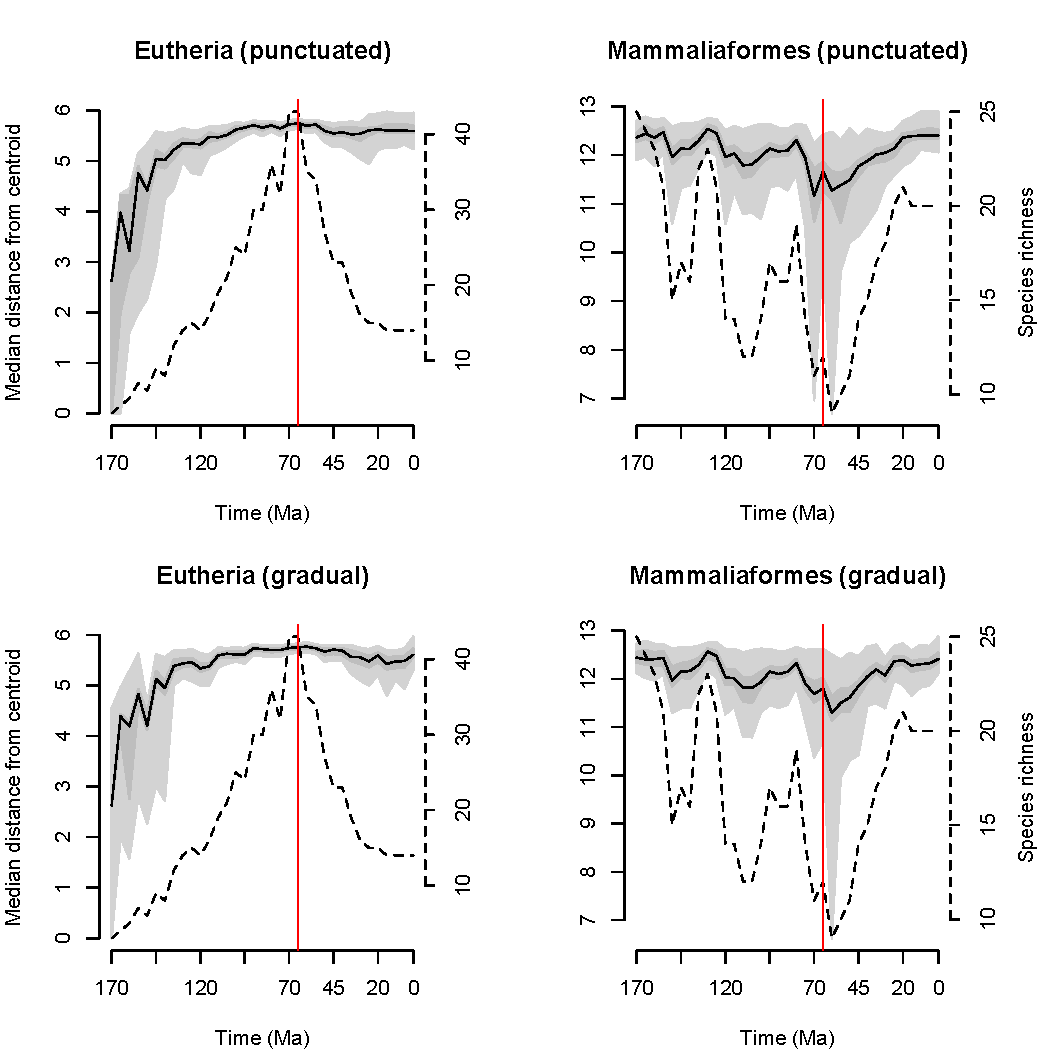
\includegraphics[keepaspectratio=true]{Figures/Main_results.pdf}
\caption{Observed variations of disparity through time among Eutherian and Mammaliaformes with a punctuated or gradual evolution model. The x axis represents the time in Million of years ago (Mya). The y axis represents the disparity measured as the median distance from centroid per sub-sample. The solid black lines is the mean disparity; the confidence intervals (CI) are represent by the grey polygons (50\% CI in dark grey and 95\% CI in light grey). The dashed line represent the species richness in each sub-sample (values are reported on the right hand side of each graphs). The red vertical line represents the K-Pg boundary (66 Mya).}
\label{fig:Fig_Raw_results}
\end{figure}

\begin{figure}[!htbp]
\centering
    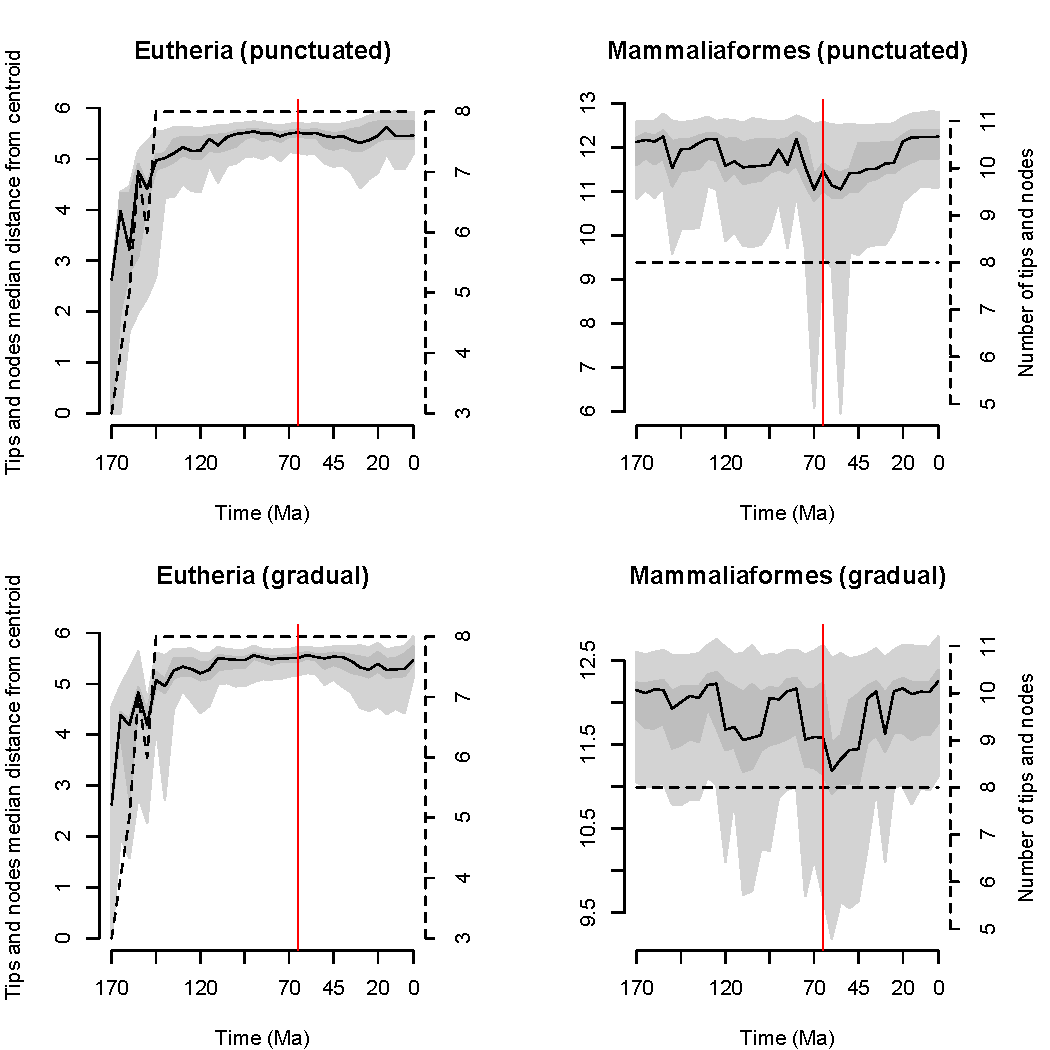
\includegraphics[keepaspectratio=true]{Figures/Main_results_rarefied.pdf}
\caption{Rarefied variations of disparity through time among Eutherian and Mammaliaformes with a punctuated or gradual evolution model. The x axis represents the time in Million of years ago (Mya). The y axis represents the disparity measured as the median distance from centroid per sub-sample. The solid black lines is the mean disparity; the confidence intervals (CI) are represent by the grey polygons (50\% CI in dark grey and 95\% CI in light grey). The dashed line represent the species richness in each sub-sample (values are reported on the right hand side of each graphs). The red vertical line represents the K-Pg boundary (66 Mya).}
\label{fig:Fig_Rar_results}
\end{figure}

\begin{landscape}
\begin{table}[ht]
\caption{Permanova results of testing the effect of time on the ordinated distance matrix with 1000 permutations based on euclidean distance. Data: Eutherian \citep[data from][]{beckancient2014}; Mammaliaformes, \citep[data from][]{Slater2012MEE}. Model: evolutionary model. Significant effects are highlighted in bold: one star (*) signifies a p-value between 0.05 and 0.005; two starts between 0.005 and 0.0005 and three stars $<$ 0.0005.}
\label{tab:Tab_permanova}
\centering
\begin{tabular}{rrrcccccccc}
  \hline
 Data & model & terms & Df & Sum of squares & Mean sum of squares & F Model & $R^2$ & p-value & \\ 
  \hline
Eutherian     & gradual    & time      & 34  & 1825.92  & 53.703  & 1.5784 & 0.0769 & \textbf{0.0009}& \textbf{***} \\ 
              &            & residuals & 644 & 21911.65 & 34.024  &        & 0.9231 &  &\\ 
              & punctuated & time      & 34  & 1597.07  & 46.973  & 1.3693 & 0.0674 & \textbf{0.0009}& \textbf{***} \\ 
              &            & residuals & 644 & 22092.28 & 34.305  &        & 0.9326 &  &\\ 
Mammaliaformes & gradual    & time      & 34  & 6525.61  & 191.930 & 1.1660 & 0.0663 & \textbf{0.0009}& \textbf{***} \\ 
              &            & residuals & 558 & 91852.55 & 164.610 &        & 0.9337 &  &\\ 
              & punctuated & time      & 34  & 5741.25  & 168.860 & 1.0167 & 0.0583 & 0.2248 &\\ 
              &            & residuals & 558 & 92672.75 & 166.080 &        & 0.9417 &  &\\ 
   \hline
\end{tabular}
\end{table}
\end{landscape}


%TG: don't know why these tables are sent to the end of the document...
\begin{table}[ht]
\caption{Results of the \textit{post-hoc} t-tests for comparing the disparity at the last sub-sample of the Cretaceous (65 Mya) to all the sub-samples of the Cenozoic for the Eutherians \citep[data from][]{beckancient2014}. Sub-samples: reference sample (65 Million years ago; Mya) to Cenozoic sample (from 60 Mya to present). Gradual: gradual evolution; punctuated: punctuated evolution. Difference: mean sub-sample difference; Df: degrees of freedom; T: T statistic; p-value: adjusted p-value using Holm-Bonferroni correction. Significant differences are highlighted in bold: one star (*) signifies a p-value between 0.05 and 0.005; two starts between 0.005 and 0.0005 and three stars $<$ 0.0005.}
\label{tab:Tab_beck_raw}
\centering
\begin{tabular}{r|ccccl|ccccl}
  \hline
  Sub-samples & \multicolumn{5}{c|}{Gradual} & \multicolumn{5}{c}{Punctuated} \\
  (Mya) & Difference & Df & T & p.value & & Difference & Df & T & p.value &\\ 
  \hline
  65:60 & 0.06 & 76 & 1.055 & 1      & & 0.04 & 76 & 0.760 & 1      &\\ 
  65:55 & 0.05 & 75 & 0.999 & 1      & & 0.16 & 75 & 3.145 & \textbf{0.0310} & \textbf{*} \\ 
  65:50 & 0.15 & 68 & 2.412 & 0.2413 & & 0.08 & 68 & 1.403 & 1      &\\ 
  65:45 & 0.21 & 64 & 3.016 & \textbf{0.0478} & \textbf{*} & 0.18 & 64 & 2.685 & 0.1200 &\\ 
  65:40 & 0.18 & 64 & 2.579 & 0.1590 & & 0.13 & 64 & 2.173 & 0.4354 &\\ 
  65:35 & 0.23 & 60 & 2.840 & 0.0800 & $\cdotp$ & 0.21 & 60 & 2.962 & 0.0568 & $\cdotp$ \\ 
  65:30 & 0.27 & 57 & 2.927 & 0.0639 & $\cdotp$ & 0.29 & 57 & 3.810 & \textbf{0.0044} & \textbf{**} \\ 
  65:25 & 0.22 & 56 & 2.500 & 0.1999 & & 0.28 & 56 & 3.544 & \textbf{0.0104} & \textbf{*} \\ 
  65:20 & 0.16 & 56 & 1.922 & 0.7762 & & 0.25 & 56 & 3.117 & \textbf{0.0374} & \textbf{*}\\ 
  65:15 & 0.14 & 55 & 1.819 & 0.9670 & & 0.30 & 55 & 3.567 & \textbf{0.0098} & \textbf{**}\\ 
  65:10 & 0.14 & 55 & 1.843 & 0.9203 & & 0.42 & 55 & 4.540 & \textbf{0.0004} & \textbf{***} \\ 
  65:5  & 0.14 & 55 & 1.790 & 1      & & 0.30 & 55 & 3.377 & \textbf{0.0176} & \textbf{*} \\ 
  65:0  & 0.14 & 55 & 1.818 & 0.9692 & & 0.17 & 55 & 2.250 & 0.3705 \\ 
   \hline
\end{tabular}
\end{table}

\begin{table}[ht]
\caption{Results of the \textit{post-hoc} t-tests for comparing the disparity at the last sub-sample of the Cretaceous (65 Mya) to all the sub-samples of the Cenozoic for the rarefied Eutherians \citep[data from][]{beckancient2014}. Column heads explained same as given in table ~\ref{tab:Tab_beck_raw}.}
\label{tab:Tab_beck_rar}
\centering
\begin{tabular}{r|cccc|cccc}
  \hline
  Sub-samples & \multicolumn{4}{c|}{Gradual} & \multicolumn{4}{c}{Punctuated} \\
  (Mya) & Difference & Df & T & p.value & Difference & Df & T & p.value \\ 
  \hline
  65:60 & 0.04  & 76 & 0.218  & 1 & 0.01 & 76 & 0.064 & 1 \\ 
  65:55 & 0.04  & 75 & 0.213  & 1 & 0.14 & 75 & 0.797 & 1 \\ 
  65:50 & 0.11  & 68 & 0.553  & 1 & 0.04 & 68 & 0.224 & 1 \\ 
  65:45 & 0.15  & 64 & 0.716  & 1 & 0.13 & 64 & 0.600 & 1 \\ 
  65:40 & 0.11  & 64 & 0.544  & 1 & 0.07 & 64 & 0.358 & 1 \\ 
  65:35 & 0.15  & 60 & 0.627  & 1 & 0.12 & 60 & 0.572 & 1 \\ 
  65:30 & 0.15  & 57 & 0.636  & 1 & 0.17 & 57 & 0.772 & 1 \\ 
  65:25 & 0.10  & 56 & 0.423  & 1 & 0.16 & 56 & 0.697 & 1 \\ 
  65:20 & 0.03  & 56 & 0.131  & 1 & 0.13 & 56 & 0.555 & 1 \\ 
  65:15 & 0     & 55 & 0.005  & 1 & 0.16 & 55 & 0.674 & 1 \\ 
  65:10 & -0.01 & 55 & -0.034 & 1 & 0.27 & 55 & 1.129 & 1 \\ 
  65:5  & 0.01  & 55 & 0.029  & 1 & 0.15 & 55 & 0.640 & 1 \\ 
  65:0  & 0     & 55 & 0.005  & 1 & 0.02 & 55 & 0.071 & 1 \\
   \hline
\end{tabular}
\end{table}


\begin{table}[ht]
\caption{Results of the \textit{post-hoc} t-tests for comparing the disparity at the last sub-sample of the Cretaceous (65 Mya) to all the sub-samples of the Cenozoic for the Mammaliaformes \citep[data from][]{Slater2012MEE} under gradual evolution model. Raw data: bootstrapped data without rarefaction; Rarefied data: rarefied bootstrapped data. Other column heads explained same as given in table \ref{tab:Tab_beck_raw}.}
\label{tab:Tab_slater}
\centering
\begin{tabular}{r|cccc|cccc}
  \hline
  Sub-samples & \multicolumn{4}{c|}{Raw data} & \multicolumn{4}{c}{Rarefied data} \\
  (Mya) & Difference & Df & T & p.value & Difference & Df & T & p.value \\ 
  \hline
  65:60 & 0.49  & 19 & 0.826  & 1      & 0.26  & 19 & 0.365  & 1 \\ 
  65:55 & 0.45  & 20 & 0.734  & 1      & 0.31  & 20 & 0.428  & 1 \\ 
  65:50 & 0.13  & 21 & 0.267  & 1      & 0.03  & 21 & 0.042  & 1 \\ 
  65:45 & -0.05 & 24 & -0.109 & 1      & 0.03  & 24 & 0.051  & 1 \\ 
  65:40 & -0.22 & 25 & -0.543 & 1      & -0.08 & 25 & -0.118 & 1 \\ 
  65:35 & -0.33 & 27 & -0.858 & 1      & -0.19 & 27 & -0.321 & 1 \\ 
  65:30 & -0.37 & 28 & -0.973 & 1      & -0.21 & 28 & -0.335 & 1 \\ 
  65:25 & -0.48 & 30 & -1.358 & 1      & -0.25 & 30 & -0.394 & 1 \\ 
  65:20 & -0.69 & 31 & -2.030 & 0.6625 & -0.44 & 31 & -0.711 & 1 \\ 
  65:15 & -0.76 & 30 & -2.201 & 0.4620 & -0.53 & 30 & -0.906 & 1 \\ 
  65:10 & -0.86 & 30 & -2.666 & 0.1593 & -0.66 & 30 & -1.241 & 1 \\ 
  65:5  & -0.85 & 30 & -2.668 & 0.1585 & -0.63 & 30 & -1.197 & 1 \\ 
  65:0  & -0.86 & 30 & -2.678 & 0.1548 & -0.62 & 30 & -1.133 & 1 \\ 
   \hline
\end{tabular}
\end{table}

%---------------------------------------------
%
%       DISCUSSION
%
%---------------------------------------------

\section{Discussion}
Our results show that there is an effect of time on changes in disparity under the assumption of gradual evolution in Mammaliaformes and Eutherians as well as under the assumption of punctuated evolution for Eutherians (table \ref{tab:Tab_permanova}).
However, regardless the taxonomic level (i.e. family \textit{vs.} genus) and regardless the evolutionary model (i.e. gradual or punctuated evolution), there is no effect of the K-Pg event on mammalian disparity (Figure \ref{fig:Fig_Rar_results}).
In fact, after correcting for species richness, we did not detect any significant difference between the last sub-sample of the Cretaceous and any of the sub-samples of the Cenozoic.
This shows that, within the frame of our data set, there is no significant changes in mammalian morphological variety across the K-Pg boundary.
In fact the disparity in Eutherians seems to reach a plateau at the end of the Jurassic (150 Mya) and probably before the Middle Jurassic (170 Mya) for the Mammaliaformes.

\subsection{Effect of the K-Pg boundary on mammalian disparity}
As previously shown, disparity is likely to evolve relatively fast within a clades history \cite{Hughes20082013}.
It appears to be the same for mammals.
Differences between Gradual and Punctuated are probably due because the truth is a mix of both \cite{Hunt21042015}.

%Link to former literature

%Caveats
Our data set is limited.
There is not many species, especially at towards the present.
Both are based on Luo's dataset (that can be why they show similarities).
One can argue that placental mammals (i.e. crown eutherians) are the one radiating, not global eutherians or even more global mammaliaformes.
However, high taxonomic level is often subjective (Cartmill) and the use of both data sets allows more to test the effect of the taxonomic level (genus \textit{vs.} family).
crown-clade definition of Placentalia: Eutheria referring to the total clade of Placentalia \citep{O'Leary08022013,beckancient2014}
%But
Using the Total Evidence tree is much better timing wise and timing is really important in such a study.
Data is confirmed (or not) with other measurements in the supplementaries.

%From Wilson 2013
%My results reveal several key findings: (1) latest Cretaceous mammals, particularly metatherians and multituberculates, had a greater ecomorphological diversity than is generally appreciated, occupying regions of the morphospace that are interpreted as strict carnivory, plant-dominated omnivory, and herbivory; (2) the decline in dental-shape disparity and body-size disparity across the K/Pg boundary shows a pattern of constructive extinction selectivity against larger-bodied dietary specialists, particularly strict carnivores and taxa with plant-based diets, that suggests the kill mechanism was related to depressed primary productivity rather than a globally instantaneous event; (3) the ecomorphological recovery in the earliest Paleocene was fueled by immigrants, namely three multituberculate families (taeniolabidids, microcosmodontids, eucosmodontids) and to a lesser extent archaic ungulates; and (4) despite immediate increases in the taxonomic richness of eutherians, their much-celebrated post-K/Pg ecomorphological expansion had a slower start than is generally perceived and most likely only began 400,000 to 1 million years after the extinction event.

% Placental vs eutherian? Cartmill blogpost

\subsection{Methodology}
Through this paper, we propose several to classic ways to measure disparity.
This is how we think they improve the whole yoke.

-Using all axis
    -Does not create a subjective cut-off
-Centroid distance
    -Does not violate co-variance thingy
    -Is more decoupled from diversity 
-Time slicing:
    -Allows model choice (gradual vs. constant)
    -Allows continuous and independent sample, not based on geological ages (and therefore not based on fossil data)
%Disparity improvements
%Previous studies have calculated disparity on a subset of PCO axes \citep[e.g.][]{Brusatte12092008} but in this study we calculated it on all the available axis (i.e. the full n dimensional cladisto-space) to avoid excluding outliers.

Howevers, biases:
    -Ancestral states reconstruction can be tricky
    -Might be sensitive to sample size (but does not seem to much)
    -Link between phylogeny and cladistic disparity
%Biases:
%-internal versus terminal branches
%-ancestral states reconstruction (solved by being conservative?)
%-poor sampling of living taxa (Guillerme & Cooper)

%Therefore, the cladisto-space is likely to be more influenced by phylogeny than the morphospace \citep{Foote29111996,Wagner01011997}. However, discrete cladistic characters are still the best source for quantifying overall morphology for large and diverse groups \citep{Brusatte12092008}. % NC: Make this justification better. why does the phylogney effect matter. Should this be mentioned here at all? TG: not specially, might be something a reviewer might point out. I remember you pointing it out ;). However, STD is become fairly common these days so maybe people have accepted the idea.


%---------------------------------------------
%
%       CONCLUSION
%
%---------------------------------------------

\section{Conclusion}
When looking at pattens of diversification, it is important to look at both phylogenetic diversification (i.e. species richness) and phenotypic diversification (i.e. disparity).
%Not much stuff is happening there but we bring improvement to methods.


%---------------------------------------------

\section{Data availability and reproducibility}

\section{Acknowledgments}
Thanks to Graeme Lloyd, Andrew Jackson, Gavin Thomas and Sive Finlay for their useful comments on measuring disparity.
%Calcualtions where performed using the Lonsdale cluster maintained by the Trinity Centre for High Performance Computing and funded through grants from Science Foundation Ireland. %TG: I actually did use the cluster but only because I'm lazy and impatient. It can definitely run on a laptop (probably between one evening and one week-end running). Should I still say I used the cluster? Or will it make it sound like it's heavy calculations?

\section{Funding} % NC: Usually this is part of acknowledgments.
This work was funded by a European Commission CORDIS Seventh Framework Programme (FP7) Marie Curie CIG grant (proposal number: 321696).

 %   \citept{key} ==>>                Jones et al. (1990)
 %   \citept*{key} ==>>               Jones, Baker, and Smith (1990)
 %   \citep{key} ==>>                (Jones et al., 1990)
 %   \citepp*{key} ==>>               (Jones, Baker, and Smith, 1990)
 %   \citepp[chap. 2]{key} ==>>       (Jones et al., 1990, chap. 2)
 %   \citep[e.g.][]{key} ==>>        (e.g. Jones et al., 1990)
 %   \citepp[e.g.][p. 32]{key} ==>>   (e.g. Jones et al., p. 32)
 %   \citepauthor{key} ==>>           Jones et al.
 %   \citepauthor*{key} ==>>          Jones, Baker, and Smith
 %   \citepyear{key} ==>>             1990

\bibliographystyle{sysbio}
\bibliography{References}

% \section{supplementaries}

% \subsection{Ancestral states estimation}
% We used both the \texttt{ace} function from the R package ape v. 3.2 \citep{paradisape:2004} and the 
% \texttt{rerootingMethod} function from the R package phytools 0.4-45 \citep{phytools}. Both method perform a maximum likelihood estimation of the ancestral values and the variance of a Brownian motion process based on the re-rooting method of \citep{Yang01121995}. The two methods differ slightly in the calculation of the normalized conditional likelihoods but mainly on the way to treat missing data. We optimised the \texttt{ace} function for fast estimation by treating missing data in the matrix as an extra character (e.g. if a character has two observed tips states 0 and 1 and a third tip has missing data (NA), the ancestor of these three tips can be estimated between the three following states: 0, 1 and NA). For the \texttt{rerootingMethod}, we followed \citep{Claddis} method and treated the missing in the tips as any possible observed state (e.g. if a character has two observed tips states 0 and 1 and a third tip has missing data (NA), the third tip will be considered as multi-state (0\&1) and the ancestor of these three tips can be estimated between the two following states: 0 and 1). Both methods perform similarly but the implementation of the \texttt{ace} function has a slightly lower accuracy  but is three times faster than the one for the \texttt{rerootingMethod} function (see supplementaries).
% % NC: Some of this probably belongs in methods

% \subsubsection{Time intervals}
% We then divide our observed cladisto-spaces into sub cladisto-spaces representing the different stages of the character-space filling. For example, if at various points in time.
% %The intervals should be a compromise between the resolution and the sample size and must be "sufficiently coards that nearly all generic first and last occurenaces can be unambiguously assigned" \citep{Foote01071994}.
% Time intervals from 170Ma (Earliest Cenomanian, Late Cretaceous) to the present.
% We count all the nodes/tips present in a given time interval.
% Classic but artificially grouping data. The minimal bin size should contain at least two nodes/tips and sometime that involves having time intervals spanning accross tens of millions of years. Such long duration time intervals have no real biological meaning since it is unlikely that all of the nodes/tips present in the time interval did ever coexisted and had ever biological interactions together.

% \subsection{Diversity}
% -Diversity in living mammals
% -Diversity per interval

% \subsection{Disparity}
% -Centroid is less correlated with diversity
% -Other metrics

% \subsection{Not to be in the paper, neither in the supplementaries (methods table)}

% \begin{table}[ht]
% \caption{Comparison of Cladisto-space studies methods}
% \centering
% \begin{tabular}{cccccccc}
%   \hline
%     Date & Author      & Distance  & axis & Binning    & Disparity   & Difference & cite \\ %
%   \hline
%          & this study  & Gower     & PCO        & Time slice & centroid    & NPMANOVA?  & \\
%     2014 & Benson      &           &            & Equal bins & Wills 1994* & NPMANOVA   & \citep{bensonfaunal2014} \\
%     2014 & Brusatte    & Euclidean & PCO        &            &             &            & \citep{brusattegradual2014} \\
%     2014 & Benton      & Euclidean & PCO        & Biostrat   & Wills 1994* & NPMANOVA   & \citep{bentonmodels2014} \\
%     2013 & Hopkins     &           &            & Equal bins & Wills 1994* &            & \citep{hopkinsdecoupling2013} \\             
%     2013 & Ruta        & GED       & 10 first   & Biostrat   & Wills 1994* & NPMANOVA   & \citep{ruta2013} \\
%     2013 & Hughes      & Euclidean &            & Biostrat   & Sum of var  &            & \citep{Hughes20082013} \\
%     2013 & Toljagic    & Euclidean & 90\% var   & Biostrat   & Wills 1994* & NPMANOVA   & \citep{toljagictriassic-jurassic2013} \\
%     2012 & Brusatte    & Euclidean & 90\% var   & Biostrat   & Wills 1994* & CI overlap & \citep{brusattedinosaur2012} \\
%     2012 & Anderson    & Gower     & PCO        &            &             &            & \citep{anderson2012using} \\
%     2010 & Prentice    & Euclidean & PCO        & Biostrat   & Wills 1994* & NPMANOVA   & \citep{prentice2011} \\
%     2011 & Thorne      & Euclidean &            & Biostrat   &             & NPMANOVA   & \citep{thorneresetting2011} \\
%     2010 & Cisneros    & Euclidean & PCO        & Biostrat   & Wills 1994* & NPMANOVA   & \citep{cisneros2010} \\
%     2008 & Brusatte    & Euclidean & 90\% var   & Biostrat   & Wills 1994* & NPMANOVA   & \citep{brusatte50} \\
%     2008 & Brusatte    & Euclidean & 90\% var   & Biostrat   & Wills 1994* & NPMANOVA   & \citep{Brusatte12092008} \\
%     2005 & Wesley-Hunt &           & PCO        &            & Foote 1992  & t-test     & \citep{Wesley-Hunt2005} \\
%   \hline
% \end{tabular}
% \end{table}
% * The 4 sum and product of range and variance


\end{document}
